\renewcommand{\thechapter}{HS}
\chapter*{Homework Solutions}
\addtocounter{chapter}{1} % Manually increment the chapter counter
\markboth{\sffamily\normalsize\bfseries Homework Solutions}{} % Set the chapter header
\addcontentsline{toc}{chapter}{\textcolor{ocre}{Homework Solutions}}
\setcounter{section}{0}

\section{Homework \#1 Solutions}

\begin{enumerate}
    \item We are given the relation $\sim$ on $\R$:  
          \[
          \forall \ r,s \in \R, \quad r \sim s \iff r - s \in \Z
          \]
          and we are to show that $\sim$ is an equivalence relation.

          \textit{Proof:}  
          \begin{enumerate}
              \item \textbf{Reflexivity:} Take $r \in \R$. Then $r - r = 0$, and $0$ is an integer, so $r \sim r$.
              \item \textbf{Symmetry:} Assume $r \sim s$. Then $r - s$ is an integer.  
              Its ``opposite'' $-(r - s)$ is also an integer, so $s - r \in \Z$ and we have $s \sim r$.
              \item \textbf{Transitivity:} Assume $r \sim s$ and $s \sim t$.  
              Then $r - s \in \Z$ and $s - t \in \Z$. The sum of two integers is again an integer, so  
              \[
              (r - s) + (s - t) \in \Z
              \]
              so $r - t \in \Z$, so $r \sim t$. $\blacksquare$
          \end{enumerate}

    \item \begin{enumerate}
              \item The equivalence class of $\pi$ is given by:
                    \[
                    \text{cl}(\pi) = \{ r \in \R \mid r \sim \pi \}
                    \]
                    which means:
                    \begin{align*}
                        \text{cl}(\pi) &= \{ r \in \R \mid r - \pi \text{ is an integer} \} \\
                        &= \{ r \in \R \mid r = ( \text{an integer} ) + \pi \} \\
                        &= \{ n + \pi \mid n \in \Z \} = \{ \dots, -1+\pi, \pi, 1+\pi, 2+\pi, \dots \}
                    \end{align*}
                    This is usually expressed as $\pi + \Z$.
                    \begin{center}
                        \hspace{-0.1in}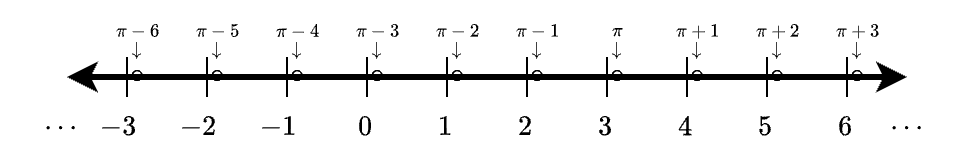
\includegraphics[width=0.85\textwidth]{Figures/EquivClassOfPiNumberLine.png}
                    \end{center}

              \item For any $s \in \R$, we can similarly find $\text{cl}(s)$ by substituting $s$ for $\pi$, so:
                    \[
                    \text{cl}(s) = s + \Z.
                    \]
                    Note that $\text{cl}(0)$ and $\text{cl}(1)$ are identical; they are both $\Z$.  
                    However, there are infinitely many $s \in \R$ between $0$ and $1$, and each such $s$ represents a class: $s + \Z$.  
                    So under the equivalence relation $\sim$ in problem (1), $\R$ is broken into infinitely many equivalence classes.
          \end{enumerate}
\end{enumerate}
% Problems 3-6
\begin{enumerate}
    \setcounter{enumi}{2}
    \item The following is an equivalence relation:  
          \[
          \forall n,m \in \Z, \quad n \sim m \iff n + m \text{ is even}.
          \]
          \textit{Proof:}  
          \begin{enumerate}
              \item \textbf{Reflexivity:} Take $n \in \Z$. Then $\underset{\substack{\ \ \ \ \ \ \ \ \ \ \ \ \ \ \ \uparrow \\ \ \ \ \ \ \ \text{the }``k" \text{ from defn. } \\
              \ \ \ \ \ \ \text{of ``even''}}}{n + n = 2n}$, which is even, so $n \sim n$.
              \item \textbf{Symmetry:} Assume $n \sim m$. Then $n + m$ is even, so there exists some $k \in \Z$ such that $n + m = 2k$.  
              Since addition in $\Z$ is commutative (i.e. $n+m=m+n$), we have $m + n = 2k$, which shows $m + n$ is even. Thus, $m \sim n$.
              \item \textbf{Transitivity:} Assume $n \sim m$ and $m \sim p$.  
              Then $\exists \ k \in \Z \ni $ $n + m = 2k$, and $\exists \ l \in \Z \ni $$m + p = 2l$.  
              Now,
              \[
              n + p = (2k - m) + (2l - m) = 2(k - m + l).
              \]
              Since $k, m, l$ are integers, $(k-m+l)$ is an integer, so $n+p$ is even, and $n \sim p$. $\blacksquare$
          \end{enumerate}

    \item Take $n \in \Z$; $n$ is either even or odd.  
          \begin{itemize}
              \item If $n$ is even, then $n + m$ is even $\iff m$ is even.  
              Since any even integer can be used for $m$, we have:
              \[
              \text{cl}(\text{any even } n) = 2\Z, \quad \text{the even integers.}
              \]
              \item If $n$ is odd, then $n + m$ is even $\iff m$ is odd.  
              This makes:
              \[
              \text{cl}(\text{any odd } n) = 1 + 2\Z, \quad \text{the odd integers.}
              \]
          \end{itemize}
          So the relation $\sim$ in (3) breaks $\Z$ into two classes: $2\Z$ and $1 + 2\Z$.

    \item Given $\sigma: \mathbb{R} \to \mathbb{Z}$ where $\sigma(r)$ is the smallest integer greater than or equal to $r$.  
          \[
          \sigma \text{ is not a bijection because it is not injective:}
          \]
          \[
          \frac{1}{2} \neq \frac{3}{4}, \text{ but } \sigma\left(\frac{1}{2}\right) = \sigma\left(\frac{3}{4}\right) = 1.
          \]

    \item Given $\alpha, \beta, \gamma: S \to S$ with $\gamma$ bijective, prove that $\alpha \circ \gamma = \beta \circ \gamma \implies \alpha = \beta$.  \\
          \textit{Proof:}  
          
              Since $\gamma$ is bijective, by L 1.2.3 $\exists$ $\gamma^{-1}: S \to S \ \ni \ \gamma \circ \gamma^{-1} = \gamma^{-1} \circ \gamma = I_S$. \\
              By hypothesis, $\alpha \circ \gamma = \beta \circ \gamma$ ; \ 
              Compose both sides with $\gamma^{-1}$ on the right:
                    \[
                    (\alpha \circ \gamma) \circ \gamma^{-1} = (\beta \circ \gamma) \circ \gamma^{-1}.
                    \]
              By associativity of composition (L 1.2.1) we can shift brackets:
              \begin{align*}
                &\alpha \circ (\gamma \circ \gamma^{-1}) = \beta \circ (\gamma \circ \gamma^{-1}). &\\
                \iff &\alpha \circ I_S = \beta \circ I_S & (\text{since }\gamma \circ \gamma^{-1} = I_S) \\
                \iff &\alpha = \beta. \ \ \ \ \ \blacksquare &
              \end{align*}
                    
              (For the last step, note that $\forall \ s\in S, (\alpha \circ I_S)(s) = \alpha[I_S(s)]=\alpha(s)$, so $\alpha \circ I_s = \alpha$. Likewise, $\beta \circ I_s =\beta$.)
          
\end{enumerate}


\newpage

\section{Homework \#2 Solutions}